\documentclass[12pt,a4paper]{article}
\usepackage[utf8]{inputenc}
\usepackage{amsmath}
\usepackage{amsfonts}
\usepackage{amssymb}
\usepackage{graphicx}
\usepackage[left=2cm,right=2cm,top=2cm,bottom=2cm]{geometry}
\author{Prabhat B}
\begin{document}

\section{Prabhat ME20B132}

\begin{equation}
\nabla\times\vec{B} = \mu_0\vec{B} + \mu_0\epsilon_0 \frac{\partial \vec{E}}{\partial t}
\label{eqn:maxwell4}
\end{equation}

Eqn.~\ref{eqn:maxwell4} is commonly known as Maxwell's fourth electromagnetic equation. It is an expansion on Amp\`{e}re's Circuital Law and is hence also known as the Amp\`{e}re-Maxwell Law. Currently a more generalized form is used, which takes into account the behaviour and interference of material substances in eletric and magnetic fields \cite{Gratus2020}.

\subsection{Terms used in the equation}
\begin{itemize}
\item $\nabla\times$ - Curl Operator
\item $\vec{B}$ - Magnetic Field Vector
\item $\vec{J}$ - Current Density Vector
\item $\vec{E}$ - Electric Field Vector
\item $\mu_0$ (Constant) - Permeability of Free Space
\item $\epsilon_0$ (Constant) - Permittivity of Free Space
\end{itemize}

It is an important equation as it links two phenomena, which were previously thought to be separate, magnetism and electricity. It also finally proved that light is an electromagnetic wave, (as seen in Fig.~\ref{fig:light} taken from a paper by J. Gratus, M.W.McCall and P.Kinsler ~\cite{Gratus2020}) leading to a whole new area and direction of research.

\begin{figure}[h]
\centerline{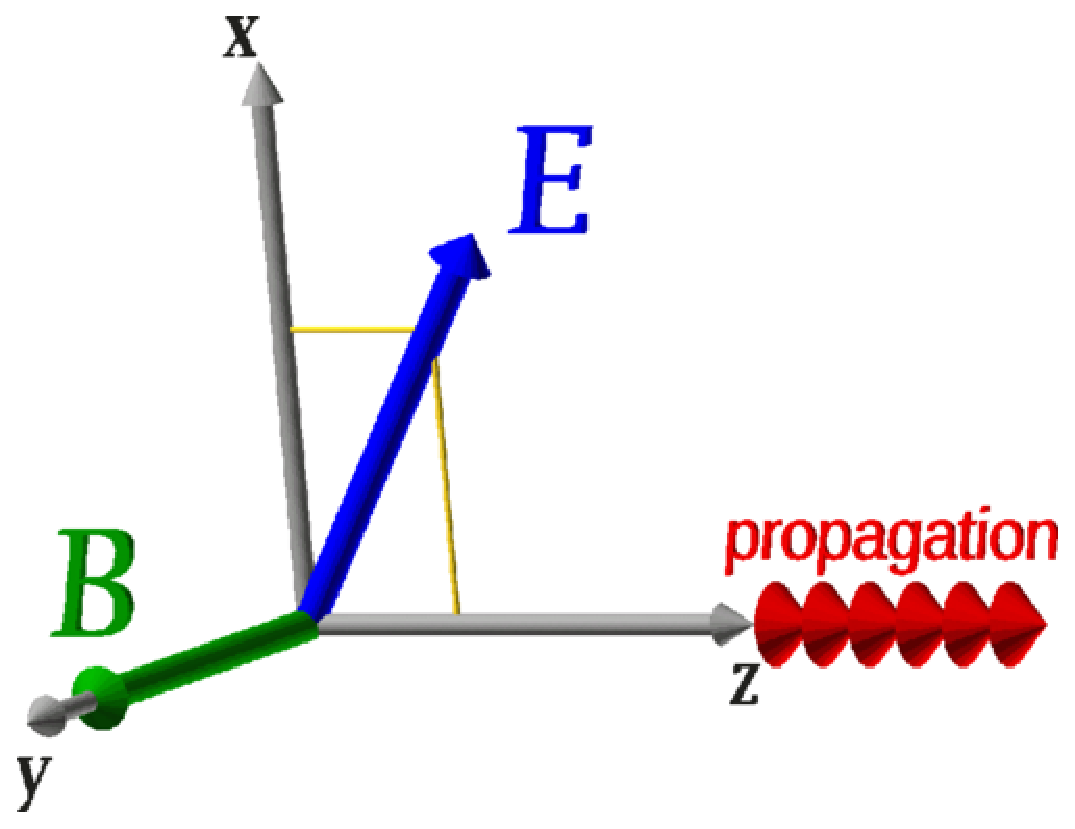
\includegraphics[width=200px,height=200px]{me20b132.eps}}
\label{fig:light}
\end{figure} 

\bibliography{me20b132}
\bibliographystyle{plain}

\end{document}